% Created 2021-02-24 Wed 09:41
% Intended LaTeX compiler: pdflatex
\documentclass{beamer}\usepackage{listings}
\usepackage{color}
\usepackage{amsmath}
\usepackage{array}
\usepackage[T1]{fontenc}
\usepackage{natbib}
\lstset{
keywordstyle=\color{blue},
commentstyle=\color{red},stringstyle=\color[rgb]{0,.5,0},
literate={~}{$\sim$}{1},
basicstyle=\ttfamily\small,
columns=fullflexible,
breaklines=true,
breakatwhitespace=false,
numbers=left,
numberstyle=\ttfamily\tiny\color{gray},
stepnumber=1,
numbersep=10pt,
backgroundcolor=\color{white},
tabsize=4,
keepspaces=true,
showspaces=false,
showstringspaces=false,
xleftmargin=.23in,
frame=single,
basewidth={0.5em,0.4em},
}
\usepackage{natbib, dsfont, pgfpages, tikz,amssymb, amsmath,xcolor, mathrsfs}
\bibliographystyle{abbrvnat}
% New operators and commands
\newcommand{\Z}{\mathbb{Z}}
\newcommand{\Q}{\mathbb{Q}}
\newcommand{\R}{\mathbb{R}}
\newcommand{\N}{\mathbb{N}}
\newcommand{\C}{\mathbb{C}}
\renewcommand{\S}{\mathbb{S}}
\newcommand{\blank}{\makebox[1ex]{\textbf{$\cdot$}}}
\newcommand\independent{\protect\mathpalette{\protect\independenT}{\perp}}
\def\independenT#1#2{\mathrel{\rlap{$#1#2$}\mkern2mu{#1#2}}}
\renewcommand{\phi}{\varphi}
\renewcommand{\epsilon}{\varepsilon}
\newcommand*\diff{\mathop{}\!\mathrm{d}}
\newcommand{\weakly}{\rightsquigarrow}
\newcommand\smallO{
  \mathchoice
    {{\scriptstyle\mathcal{O}}}% \displaystyle
    {{\scriptstyle\mathcal{O}}}% \textstyle
    {{\scriptscriptstyle\mathcal{O}}}% \scriptstyle
    {\scalebox{.6}{$\scriptscriptstyle\mathcal{O}$}}%\scriptscriptstyle
}
\newcommand{\midd}{\; \middle|\;}
\newcommand{\1}{\mathds{1}}
\usepackage{ifthen} %% Empirical process with default argument
% \newcommand{\G}[1][]{%
%    \ifthenelse{ \equal{#1}{} }
%       {\ensuremath{\mathbb{G}_n}}
%       {\ensuremath{\mathbb{G}_{#1}}}
% }
% New version:
\newcommand{\G}[2][n]{
{\ensuremath{\mathbb{G}_{#1}}{\left[#2\right]}}
}
\DeclareMathOperator*{\argmin}{\arg\!\min}

% New operators for consistent notation
\newcommand{\V}{\mathrm{Var}} % variance
\newcommand{\measure}[1]{\mathrm{{#1}}} % measure
% \newcommand{\measure}[1]{\textnormal{\textbf{{#1}}}} % measure
\newcommand{\m}[1]{\measure{#1}} % measure shortcut
\newcommand{\eqd}{\stackrel{d}{=}} % equality in distribution
\newcommand{\arrow}[1]{\xrightarrow{\; {#1} \;}}
\newcommand{\arrowP}{\xrightarrow{\; \m{P} \;}} % convergence in probability
\newcommand{\leb}{\lambda} % the Lebesgue measure
\newcommand{\T}{\top} % transpose
\newcommand{\KL}{\ensuremath{D_{\mathrm{KL}}}}

\usepackage{xargs}
% Make it easy to change counterfactual notation:
\newcommandx{\cf}[4][3={}, 4={}]{
  % \ifthenelse{ \equal{#4}{} }
  % {{#1^{#2}}(#3)}
  {\ifthenelse{ \equal{#3}{} }
    {{#1^{#2}}_{#4}}
    {{#1^{#2}}_{#4}(#3)}}
}

% Easily change notation:
\DeclareMathOperator{\TT}{\Psi} % target parameter
\newcommand{\lp}{\mathcal{L}_{\P}^2} % shortcut for lp2 space
\newcommand{\empmeas}{\hat{\mathbb{P}}_n} % empirical measure
\DeclareMathOperator{\E}{\mathbb{E}} % expectation
\renewcommand{\P}{\m{P}} % probability
\newcommand{\ic}{\mathrm{IF}} % influence curve
\setbeamertemplate{footline}[frame number]
\beamertemplatenavigationsymbolsempty
\usepackage{appendixnumberbeamer}

\renewcommand*\familydefault{\sfdefault}
\itemsep2pt
\usepackage[utf8]{inputenc}
\usepackage[T1]{fontenc}
\usepackage{graphicx}
\usepackage{grffile}
\usepackage{longtable}
\usepackage{wrapfig}
\usepackage{rotating}
\usepackage[normalem]{ulem}
\usepackage{amsmath}
\usepackage{textcomp}
\usepackage{amssymb}
\usepackage{capt-of}
\usepackage{hyperref}
\usetheme{default}
\author{Anders Munch}
\date{February 24, 2021}
\title{Journal club: Boosted nonparametric hazards with time-dependent covariates}
\begin{document}

\maketitle
\begin{frame}[label={sec:orgd4cd4a9}]{The article}
\begin{center}
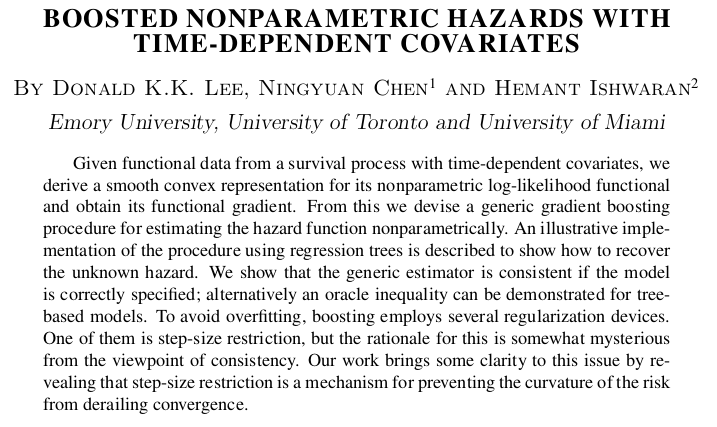
\includegraphics[width=.9\linewidth]{./screenshots/Screenshot_abstract.png}
\end{center}

To appear in Annals of Statistics. 
\end{frame}

\begin{frame}[label={sec:org3b136f7}]{Outline of the problem}
\begin{quote} %% no non-par methods quote
While there are many \alert{boosting methods} for dealing with time-static covariates, the literature is
far more sparse for the case of time-dependent covariates. In fact, to our knowledge there is \alert{no
general nonparametric approach for dealing with this setting}. This is because in order to implement
a fully nonparametric estimator, one has \alert{to contend with the issue of identifying the gradient,
which turns out to be a non-trivial problem due to the functional nature of the data}. This is
unlike most standard applications of gradient boosting where the gradient can easily be identified
and calculated. (p.2)
\end{quote}
\end{frame}

\begin{frame}[label={sec:orgae00579}]{Setting and motivation -- why?}
\begin{block}<+->{Their setting}
\begin{center}
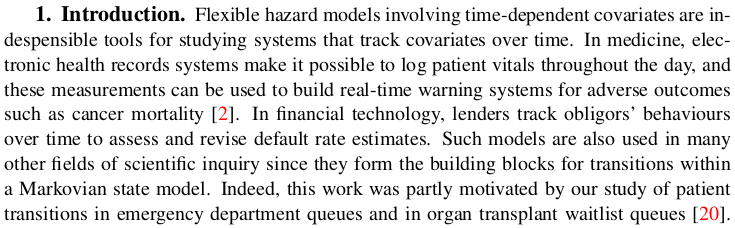
\includegraphics[width=.9\linewidth]{./screenshots/Screenshot_motivation.png}
\end{center}
\end{block}

\begin{block}<+->{Nuisance / plug-in estimator}
\begin{itemize}
\item mediation analysis in continuous time
\item dynamic treatment regime in continuous time
\item local independence testing
\end{itemize}
\end{block}
\end{frame}

\begin{frame}[label={sec:org9363528}]{Boosting in general (regression and classification)}
\pause
\begin{block}<+->{Fitting residuals}
Initialize $f_0 = \bar{y_i}$, then iteratively estimate $f_m$ to minimize
\begin{equation*}
  \frac{1}{n}\sum_{i=1}^{n}(r_{im} - f_m(x_i))^2 \quad \text{with} \quad r_{im} := y_i - f_{m-1}(x_i).
\end{equation*}
\end{block}

\begin{block}<+->{Re-weighting samples}
Initialize weights \(w_i = 1/n\), \(i = 1, ..., n\), then repeat
\begin{enumerate}
\item fit \(f_m\) to weighted data set
\item update weight \(w_i\) based on \(f_m\)'s performance on sample \(i\)
\end{enumerate}
\end{block}

\begin{block}<+->{\(\rightarrow\) Functional gradient descent of some loss function \(L\)}
\vspace{-0.5cm}
\begin{equation*}  
  F_m = F_{m-1} - v f_m, \quad \text{with} \quad  f_m = \argmin_f \left\| \frac{\partial L}{\partial F} \bigg\rvert_{F=F_{m-1}} -f \right\|
\end{equation*}
\end{block}
\end{frame}

\begin{frame}[label={sec:org734afa0}]{The loss function in this setting}
\begin{center}
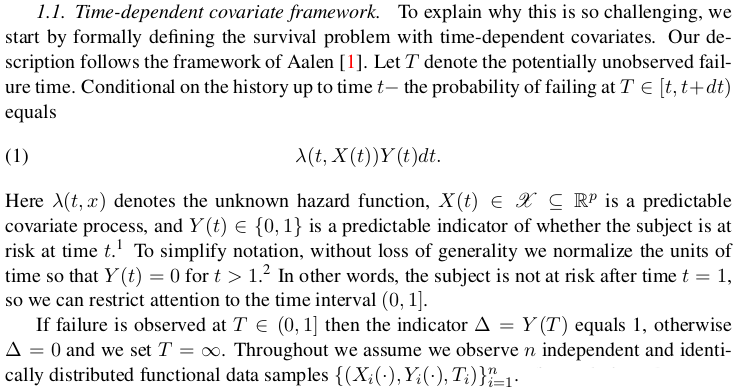
\includegraphics[width=.9\linewidth]{./screenshots/Screenshot_time-dependent-covar2.png}
\end{center} \pause
\begin{block}{The (scaled) negative log-likelihood functional}
\vspace{-0.5cm}
\begin{equation*}
  \hat{R}_n(F) = \frac{1}{n}\sum_{i}^{n}\int_0^1 Y_i(t)e^{F(t, X_i(t))} \diff t
  - \frac{1}{n}\sum_{i=1}^{n}\Delta_i F(T_i, X_i(T_i)),
\end{equation*}
where $F(t,x) = \log(\lambda(t,x))$ and $\Delta_i$ is event indicator. 
\end{block}
\end{frame}

\begin{frame}[label={sec:orgaec59e5}]{\(\hat{R}_n\) does not have a gradient \ldots{} ?}
\begin{center}
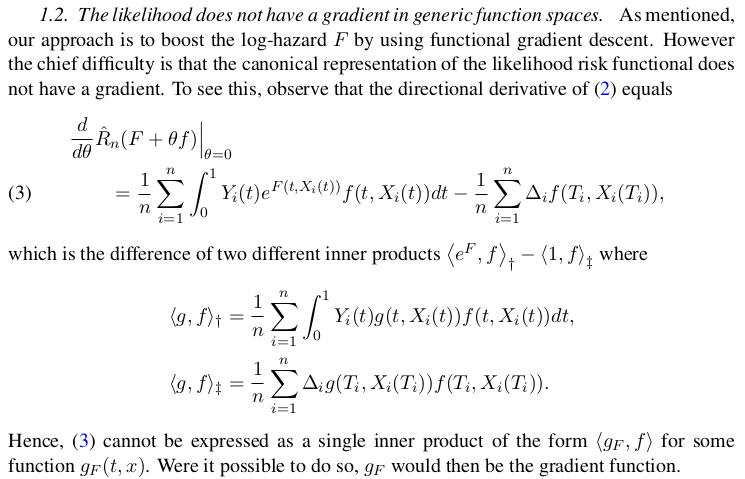
\includegraphics[width=.9\linewidth]{./screenshots/Screenshot_gradient.png}
\end{center}
\end{frame}

\begin{frame}[label={sec:org732c07e}]{Finding a domain for \(\hat{R}_n\)}
Let $\hat{\mu}_n$ be the empirical sub-probability measure on $[0,1] \times \mathscr{X} \subset
[0,1] \times \R^p$, defined as
\begin{equation*}
  \hat{\mu}_n(B) := \frac{1}{n}\sum_{i=1}^{n}\int_0^1 Y_i(t) \cdot I[\{t, X_i(t)\} \in B] \diff t,
\end{equation*}
let $\{\phi_j(t,x)\}_{j=1}^d$ be a set of bounded functions
\begin{equation*}
  \phi_j \colon [0,1] \times \mathscr{X}  \rightarrow [-1,1],
\end{equation*}
that are linearly independent in $\mathcal{L}^2(\diff t \otimes \diff x)$, and set
\begin{equation*}
  \mathcal{F} := \mathrm{span}\{\phi_j \; : \; j = 1, \dots, d\}.
\end{equation*}
Then the sample-dependent
domain of $\hat{R}_n$ is
\begin{equation*}
  (\mathcal{F}, \langle\blank, \blank\rangle_{\hat{\mu}_n}) \subset \mathcal{L}^2(\hat{\mu}_n).
\end{equation*}
\end{frame}

\begin{frame}[label={sec:org3e58cce}]{The domain when using regression trees}
\begin{center}
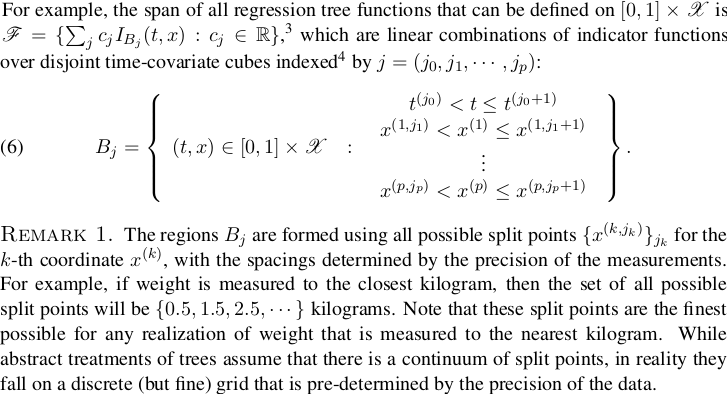
\includegraphics[width=.9\linewidth]{./screenshots/Screenshot_basis-trees.png}
\end{center}
\end{frame}

\begin{frame}[label={sec:org46f5801}]{Integral representation of the likelihood}
\begin{center}
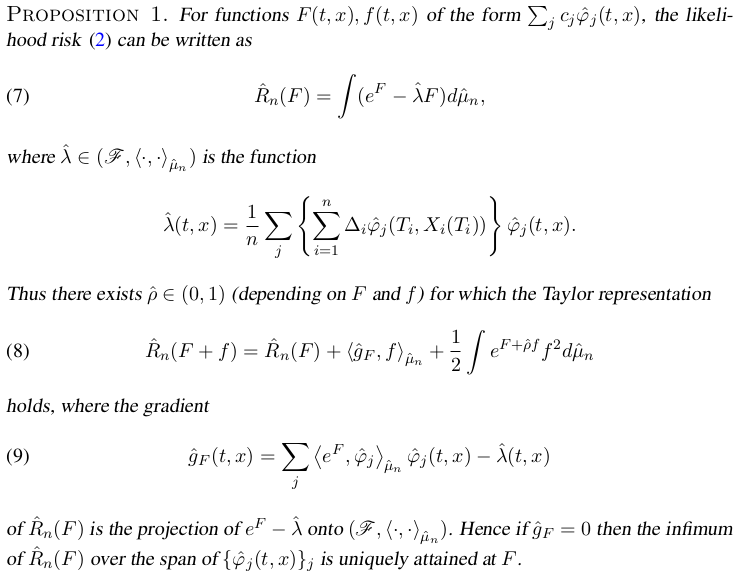
\includegraphics[width=.9\linewidth]{./screenshots/Screenshot_proposition1.png}
\end{center}
\end{frame}

\begin{frame}[label={sec:org065597a}]{Representation for regression trees}
\begin{center}
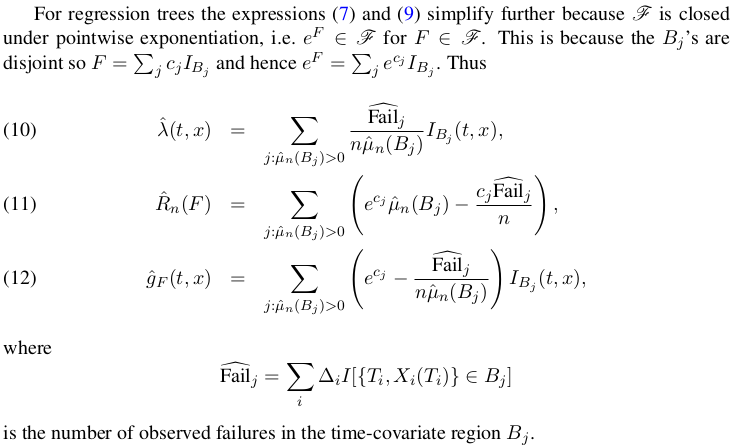
\includegraphics[width=.9\linewidth]{./screenshots/Screenshot_prop1-trees.png}
\end{center}
\end{frame}

\begin{frame}[label={sec:orgd9aa7e6}]{The boosting algorithm}
\begin{center}
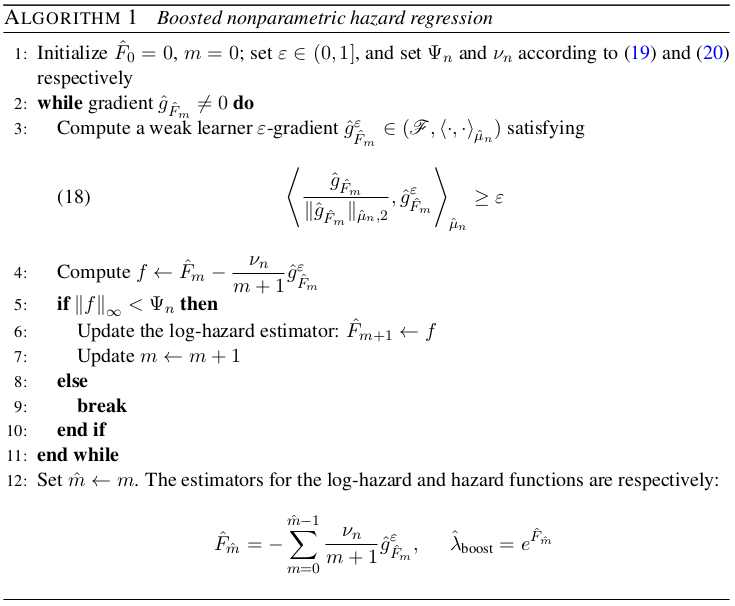
\includegraphics[width=.9\linewidth]{./screenshots/Screenshot_algorithm.png}
\end{center}
\end{frame}

\begin{frame}[label={sec:org8faf8e4}]{Skipping some technical stuff}
\begin{itemize}
\item Consistency
\item Convergence rates
\item Choice of hyper-parameters
\item Better understanding of boosting in general
\end{itemize}
\end{frame}
\begin{frame}[label={sec:orgbdd7121}]{Some details for a tree-based implementation}
At the $m$'th iteration approximate the gradient $\hat{g}_{\hat{F}_m}$ with a tree: Split leaf
regions $A \subset [0,1] \times \mathscr{X}$ into left and right daughter sub-regions $A_1$ and
$A_2$, either by splitting on a covariate $k$,
\begin{equation*}
  A_1 = \{(t, x) \in A \; : \; x^{(k)} \leq s\}, \quad   A_2 = \{(t, x) \in A \; : \; x^{(k)} > s\},
\end{equation*}
or on time
\begin{equation*}
  A_1 = \{(t, x) \in A \; : \; t \leq s\}, \quad   A_2 = \{(t, x) \in A \; : \; t > s\}.
\end{equation*}
\pause Choosing these to minimize $\mathcal{L}^2(\hat{\mu}_n)$ error is equivalent to minimizing
\begin{equation*}
  \min_{\gamma_1} \sum_{\substack{j: B_j \subseteq A_1, \\ w_j > 0}} w_j \cdot (\tilde{y}_j - \gamma_1)^2
  +   \min_{\gamma_2} \sum_{\substack{j: B_j \subseteq A_2, \\ w_j > 0}} w_j \cdot (\tilde{y}_j - \gamma_2)^2,
\end{equation*}
where
\begin{equation*}
  \tilde{y}_j := e^{c_{m,j}} - \frac{\hat{\mathrm{Fail}}_j}{n \hat{\mu}_n(B_j)}, \quad \text{and}
  \quad w_j := \hat{\mu}_n(B_j),
\end{equation*}
are the pseudo-response and its weight. 
\end{frame}

\begin{frame}[label={sec:org35b1ff2}]{Simulations}
\begin{onlyenv}<1>
\begin{center}
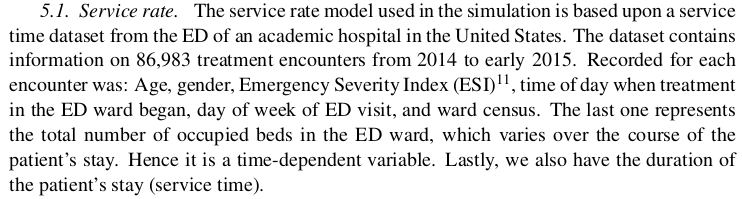
\includegraphics[width=.9\linewidth]{./screenshots/Screenshot_sim1.png}
\end{center}

Use some exploratory analysis to find a suitable, realistic functional form of the hazard.
\end{onlyenv}

\begin{onlyenv}<2>
\begin{center}
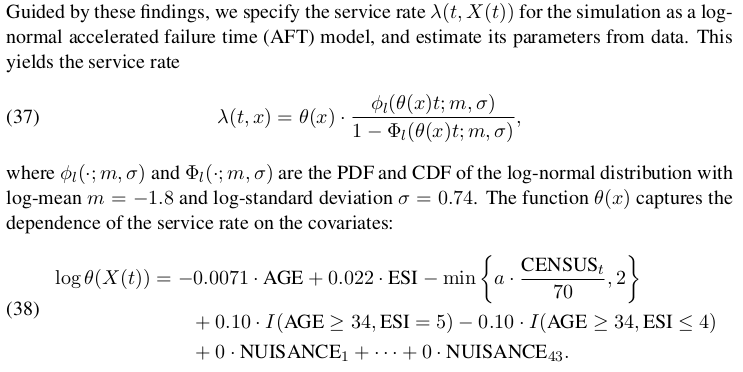
\includegraphics[width=.9\linewidth]{./screenshots/Screenshot_sim2.png}
\end{center}    
\end{onlyenv}
\end{frame}

\begin{frame}[label={sec:org7adeee3}]{Results}
\begin{center}
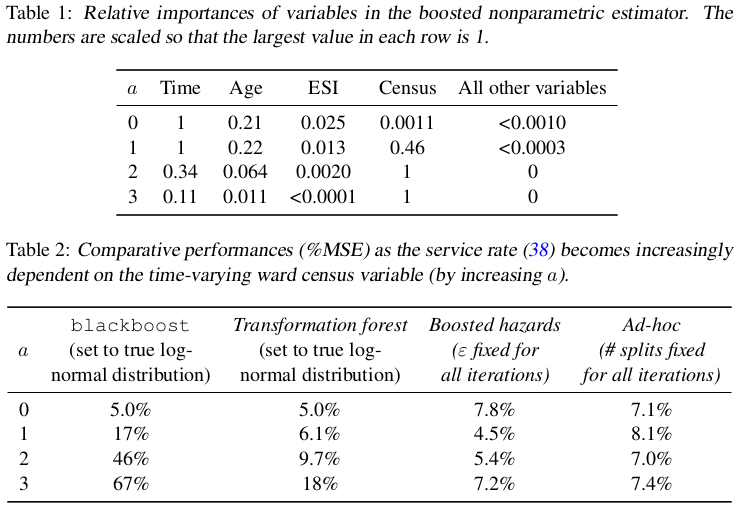
\includegraphics[width=.9\linewidth]{./screenshots/Screenshot_results.png}
\end{center} 
\end{frame}

\begin{frame}[label={sec:org7e19044}]{Summary}
\begin{itemize}
\item First (?) general method for non-parametric conditional hazard estimation
\item Finding the proper domain for the log-likelihood and an integral representation for its derivative
\item Should discuss the Markov-like assumption and the time/measurement splitting
\end{itemize}
\end{frame}
\end{document}